\part{Minerando}
\label{ch:capitulo5}
\chapter*{Minerando}
%O processo de jogar na loteria da prova de trabalho para ganhar o direito de escrever na livro de registros do Bitcoin é popularmente conhecido como mineração e é assim que funciona:
O processo de jogar na loteria de Prova de Trabalho para ganhar acesso e escrever o livro razão do Bitcoin é popularmente conhecido como \textit{mineração}.
Agora estamos prontos para ver como a loteria de prova de trabalho do Bitcoin realmente funciona:

\begin{enumerate}
\item Qualquer pessoa que desejar participar, entra na rede Bitcoin conectando seu computador e ouve as transações;
\item Ana anuncia sua intenção de enviar algumas moedas para Bruno. Os computadores da rede ficam conversando entre si para espalhar essa transação para todos demais usuários;
\item Todos os computadores que desejam participar da loteria começam a fazer o hash das transações que ouviram falar, acrescentando os nonces aleatórios à transação e executando as funções do hash sha256;
\item Aproximadamente a cada dez minutos, algum computador a encontra um número hash menor que o número alvo atual ganha a loteria;
\item Este computador anuncia o número vencedor que eles encontraram e a entrada (transações e nonce) que eles usaram para produzi-lo. Pode ter levado horas para conseguir, ou alguns minutos. Essas informações juntas (transações, nonce e hash da Prova de Trabalho) são chamadas de \textit{bloco};
\item Todos os outros validam o bloco verificando se as transações junto com o nonce do hash de fato geram aquele determinado hash, e se ele é de fato menor que o \textit{Número Alvo} e se o bloco não contém nenhuma transação inválida, e que a história dentro dele não conflita com blocos anteriores;
\item Todos escrevem o bloco em sua cópia do livro-razão, acrescentando-o à cadeia de blocos existente, produzindo uma \textit{blockchain}.
\end{enumerate}

É isso. Produzimos nosso primeiro bloco e nossa primeira entrada em nossos livros-razão.
Talvez você já tenha lido em algum lugar da mídia que minerar Bitcoins envolve solucionar equações complexas. Agora você entende que isso é falso. Invés de solucionar equações, a loteria de mineração de Bitcoin é sobre jogar um dado gigante repetidas vezes para produzir um hash dentro de um dado intervalo. É simplesmente um jogo de azar, que força os participantes a gastarem uma certa quantia de eletricidade. %

\paragraph{Como são minerados novos bitcoins?}
\paragraph{}

Até agora, discutimos como Ana pode enviar R\$2,00 para Bruno. Vamos parar de falar em reais, porque o Bitcoin não sabe nada sobre essa moeda. O que temos são os próprios bitcoins - unidades digitais que representam valor na rede Bitcoin.

Para revisitar nosso exemplo, o que realmente está acontecendo é que Ana está enviando 2 bitcoins para Bruno, anunciando que ela está movendo bitcoins que estão registrados na sua “conta” para a conta de Bruno. Alguém então ganha na loteria de Prova de Trabalho e escreve sua transação no livro-razão.

Mas onde Ana conseguiu esses 2 bitcoins para começo de conversa? Como o Bitcoin começou e como alguém adquiriu o Bitcoin antes de haver lugares para comprá-lo com a moeda fiduciária tradicional, como o real brasileiro?

%faltou esse paragrafo
Quando Satoshi criou o Bitcoin, ele podia ter criado um banco de dados no qual ele seria o dono de 21 milhões de moedas e pedido a pessoas comprarem isso dele. Porem, teria-se pouco motivo para pessoas atribuírem valor a um sistema que apenas uma pessoa controla toda a riqueza. Ele poderia criar um registro, onde algumas pessoas poderiam se cadastrar com um e-mail para ter uma chance de ganhar algumas moedas, mas isso seria suscetível a um ataque de Sybil(impersonificação) visto que da para gerar milhões de endereços de e-mails quase que gratuitamente.

Acontece que o processo de mineração de bitcoin, que é o processo de jogar na loteria de Prova de Trabalho e obter direitos de acesso ao livro-razão, é exatamente o que produz mais unidades de bitcoin. Quando você encontra um bloco válido (utilizando uma grande quantidade de energia e encontrando um número que é válido e que te faz vencedor da loteria), você pode escrever todas as transações sobre as quais ouviu falar naquele Bloco e, portanto, no livro-razão.

Mas você também pode gravar uma transação adicional muito especial, chamada de transação \textit{coinbase} (ou transação de cunhagem no português) no livro-razão. Essa transação basicamente diz: "12,5 Bitcoins foram criados e dados a Maria, a mineradora, para compensá-la por gastar toda aquela energia para minerar este bloco".

%faltou esse paragrafo
É assim que novos bitcoins são minerados a existência. esse processo permite absolutamente qualquer pessoa no mundo de minerar seus próprios bitcoins sem a existência de uma autoridade central, e sem identificar a eles mesmos, contanto que estejam dispostos a pagar pelo custo da eletricidade necessário para participar da loteria. Isso torna Bitcoin resistente a ataque de Sybil. Se você quiser moedas terás que gastar energia e pagar um dinheiro para minerar elas.

\paragraph{A recompensa do bloco}
\paragraph{}

Assim, a pessoa que ganha na loteria pode dar a si mesma alguns bitcoins recém criados. Mas por que 12,5 bitcoin e não 1000? Por que ela não pode enganar o sistema e dar a si mesma qualquer quantia? 

Aqui está a parte principal: O Bitcoin é um sistema de consenso distribuído. Isso significa que todos devem concordar sobre o que é válido. A maneira que se faz isso é através de rodar um software no computador que aplica um grupo de regras bem definidas, conhecidas como as regras de consenso do Bitcoin. Qualquer bloco produzido por mineradores é validado por essas regras. Se ele passar, todos irão escrever em seus livros razão e aceitar como a verdade. Se não o bloco é rejeitado.

embora a lista completa de regras de consentimento seja um tanto complexa, aqui estão alguns exemplos.
%adicionado
\begin{itemize}
    \item  Um bloco valido pode criar uma quantia especifica de Bitcoins, determinada pelo cronograma de emissão que esta escrito no código
    \item  Transações precisam ter assinaturas corretas, indicando que as pessoas que estão gastando aquelas moedas tem a autorização devida.
    \item Não é permitido ter transações que gastam moedas que haviam sido gastas anteriormente nesse bloco ou qualquer outro bloco anterior.
    \item A informação contida em um bloco não pode ser maior que um determinado tamanho.
    \item O hash de prova de trabalho precisa ser inferior ao atual tamanho alvo, provando a improbabilidade estatística desse bloco ter sido minerado utilizando qualquer outro método que não o gasto de uma certa quantidade de energia.
\end{itemize}
%
Se Maria criar um bloco e decidir dar a si mesma algo além desta quantidade, o computador de todos os outros \textit{rejeitará} o bloco como sendo inválido, porque dentro do software do Bitcoin Client que todos estão executando, há um trecho de código que diz "a recompensa do bloco atual é exatamente 12,5 bitcoin. Se você receber um bloco que concede a alguém mais do que isso, não aceite”.

Se Maria tentar trapacear e produzir um bloco \textit{inválido}, o bloco não será gravado no livro-razão de ninguém e ela terá desperdiçado milhares de dólares em eletricidade produzindo algo que ninguém aceitará, ou seja, uma falsificação.
%adicionado
Isso concede ao Bitcoin uma custo infalsificável(\textit{unforgeable costliness}), um termo usado primeira vez pelo pioneiro em moedas digitais, Nick Szabo, no seu artigo \textit{Shelling Out}. Intuitivamente sabemos que se dinheiro fosse fácil de falsificar, não seria muito útil como dinheiro. Bitcoin é tão impossível de se falsificar, quanto é fácil de testar, através de um simples verificação matemática.
%   
O primeiro bloco minerado foi criado por Satoshi. O código é de código aberto - isso significa que qualquer pessoa pode dar uma olhada em como ele funciona e validar que nada de suspeito está acontecendo por detrás dos panos. Até o Satoshi teve que fazer cálculos e jogar na loteria de Prova de Trabalho para extrair o primeiro bloco.%
%adicionado
Ele mesmo não poderia produzir uma falsificação, fraudando o custo de energia, embora ele seja o criador do sistema.

%adicionado
Qualquer pessoa que se juntou a rede depois dele pode verificar o hash que ele gerou com alvo inicial e os dados da transição para notar que ele havia atingindo o alvo estatisticamente raro através do gasto de energia. Imagine ser capaz de auditar a criação de dinheiro do tradicional sistema bancário fiat nesse nível de precisão e em tempo real.

\paragraph{O Halving}
\paragraph{}
%adicionado
O processo de mineração produz novos Bitcoins. Mas Satoshi queria um sistema que não era possível de ser depreciar. Ele não queria que a oferta monetária pudesse ser perpetuamente expandida. Invés, ele projetou um cronograma de emissão de novas moedas que começava muitas e tendia a zero novas moedas por ano.

No início, a recompensa do bloco era de 50 bitcoin, então foi isso que Satoshi ganhou por minerar o primeiro bloco, assim como as outras pessoas que se juntaram à rede nos primeiros dias depois dos primeiros blocos serem criados.

O código Bitcoin impõe que cada recompensa do bloco seja reduzida pela metade a cada quatro anos aproximadamente. Isso se baseia na quantidade de blocos minerados, e não na passagem do tempo, mas eles são quase os mesmos devido aos blocos sendo produzidos aproximadamente a cada dez minutos.

A Recompensa por Bloco em 2009 foi de 50, em 2012 foi de 25, em 2016 foi de 12,5. A partir de hoje, 15 de janeiro de 2019 - foram minerados 558.688 blocos, desde o início da história do Bitcoin, e a recompensa é de 12,5 bitcoin por bloco.

71.312 blocos a partir deste momento, ou aproximadamente no final de maio de 2020, a recompensa será reduzida para 6,25 bitcoins por bloco, levando a uma inflação do fornecimento anual de moedas para aproximadamente 1,8\%. Uma década depois, após dois halvings, mais de 99\% de todo o Bitcoin terá sido minerado e menos de 1 bitcoin será produzido por bloco. Você pode monitorar o processo de halving em \url{https://www.bitcoinblockhalf.com/}

\begin{figure}
  \centering
  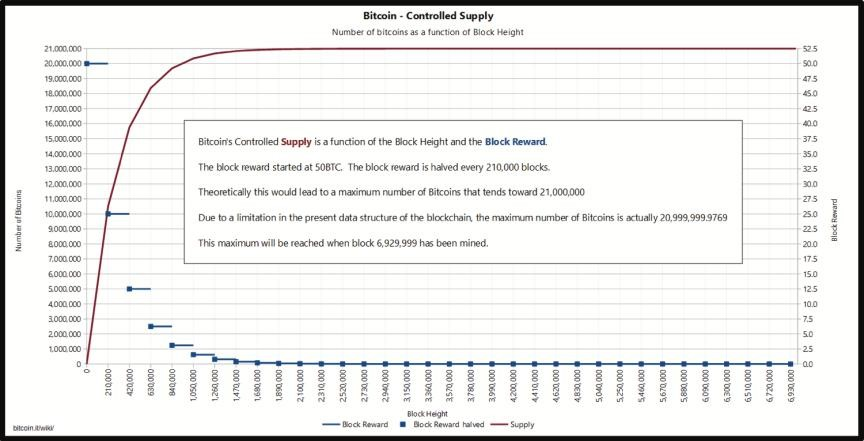
\includegraphics[width=10cm]{imagens/grafico-capitulo-05.jpg}
  \caption{\url{https://en.bitcoin.it/w/images/en/4/42/Controlled_supply-supply_over_block_height.png}}
\end{figure}

Eventualmente, por volta do ano 2140, a Recompensa por Bloco desaparecerá totalmente, e os mineradores serão incentivados apenas pelas taxas pagas por aqueles que realizam as transações.

Esses números de emissão e de recompensa de bloco são aplicados no código Bitcoin - que, para reiterar, é totalmente de código aberto e pode ser validado por qualquer pessoa - dependendo de quão longe estamos na história do Bitcoin, produzindo um bloco que não siga essas regras fará com que você seja rejeitado por todos os outros que estão verificando as mesmas que estão escritas em seus códigos.

\paragraph{Controlando a Emissão e Intervalo de Mineração}
\paragraph{}

A mineração requer hardware e eletricidade, portanto, quanto mais hardware e eletricidade você controlar, maior será a probabilidade de encontrar o resultado mais rápido, em comparação às demais pessoas. Por exemplo, se houver 100 computadores com velocidade e custo energético igual na rede e você controlar 10 deles, encontrará o bloco vencedor em \textit{aproximadamente} 10\% das vezes. No entanto, a mineração é um processo baseado no acaso e na aleatoriedade, então é possível que horas ou mesmo dias possam se passar sem que você encontre um bloco.

Como foi falado na seção anterior, os mineradores não podem simplesmente conceder a si mesmos recompensas de blocos arbitrárias, ou seriam rejeitados pelos demais nodes. Mas e se eles gastarem muita energia para adiantar os blocos de mineração e colocarem as mãos em um monte de bitcoins, violando a restrição do projeto de que o cronograma de emissão deve ser conhecido com antecedência?

Vamos novamente ao exemplo de que há apenas 1000 hashes possíveis e nosso número de alvo sendo 100. Isso significa que 10\% das vezes vamos lançar um número menor que 100 e encontrar um bloco.

Digamos que leve 1 segundo para calcular cada hash. Se a cada segundo "lançarmos nosso dado" misturando as transações atuais e nosso nonce aleatório, e 10\% das vezes atingirmos um número menor que o alvo, então esperamos que leve cerca de 10 segundos, em média, para encontrar um hash válido.

O que acontece se dois computadores estiverem apostando nessa loteria? Eles têm duas vezes mais hashes sendo tentados, então esperamos que um hash válido seja encontrado em 5 segundos. E se 10 computadores estiverem jogando? Um deles encontrará um hash válido aproximadamente a cada segundo.

Isso cria um problema: se mais pessoas estão minerando, os blocos serão produzidos muito rapidamente. Isso gera dois resultados que não queremos:

\begin{enumerate}
\item Isso atrapalha a ideia de ter um cronograma de emissão pré-determinado. Queremos que seja emitido um número relativamente consistente de bitcoins por hora para ter certeza de que emitiremos todos eles até o ano 2140, e não antes disso;
\item Isso cria problemas de rede: se os blocos são extraídos tão rapidamente que não têm tempo de alcançar toda a rede antes que o próximo seja extraído, então não podemos chegar a um consenso sobre uma história linear de transações, uma vez que vários mineradores podem incluir a mesma transação em seus blocos, fazendo com que os blocos sejam inválidos por conterem transações que já foram gastas em outros blocos.
\end{enumerate}

E se menos pessoas estão minerando, criamos o problema oposto:
\begin{samepage}
\begin{enumerate}
\item Os bitcoins estão sendo emitidos muito lentamente, novamente interferindo na emissão pré-determinada;
\item A blockchain pode se tornar inutilizável conforme as pessoas esperam horas, dias ou até mesmo semanas, para obter uma transação gravada no livro-razão.
\end{enumerate}
\end{samepage}

O número total de hashes por segundo executado por todos os mineradores da rede Bitcoin é conhecido como \textit{hash rate}.

\begin{figure}
  \centering
  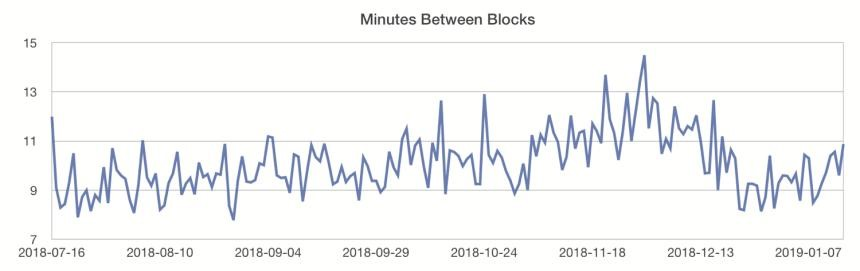
\includegraphics[width=10cm]{imagens/grafico2-capitulo-05.jpg}
  \caption{Minutos entre blocos minerados}
\end{figure}

\paragraph{Ajustes de dificuldade: concordando com a meta}
\paragraph{}
%adicionado
Como Bitcoin é um sistema voluntario e sem permissão que pessoas podem participar quando desejarem, sem ninguém comandando, o numero de mineradores ativos em um dado momento pode variar drasticamente. Precisamos de uma maneira de manter a produção de blocos estável impedindo aumentos ou reduções no cronograma toda vez que um minerador novo entra na rede ou um minerador existente saia.

Como podemos tornar mais difícil encontrar hashes válidos se mais jogadores entrarem na loteria e mais fácil se os jogadores saírem dela, a fim de manter os tempos de emissão e de blocos estáveis?

%adicionado
Lembre que mineração de Bitcoin é uma loteria para tentar produzir um numero aleatório menor que um alvo.
%faltou figura?

O Bitcoin resolve esse problema com um \textit{ajuste de dificuldade de mineração}. Como todos estão executando o mesmo código, que impõe as mesmas regras, e todos têm uma cópia de todo o histórico de blocos até este ponto, todos podem calcular de forma independente a rapidez com que os blocos estão sendo produzidos.

A cada 2016 blocos, o que leva aproximadamente o equivalente a duas semanas, olhamos para trás e descobrimos quanto tempo levou para produzir esses blocos e, em seguida, ajustamos nosso \textit{Número Alvo} para acelerar ou desacelerar a produção de blocos.

Todos os usuários pegam os últimos 2016 blocos e os dividem pelo tempo que levaram para produzir, criando assim uma média. Demorou mais de dez minutos? Estamos indo muito devagar. Demorou menos de dez minutos? Estamos indo rápido demais.

Agora podemos fazer um ajuste no \textit{Número Alvo} para que seja aumentado ou diminuído proporcionalmente a quanto mais rápido ou mais devagar queremos ir com base no intervalo de 10 minutos que está escrito no código fonte.

Podemos aumentar o \textit{Número Alvo} para um número mais alto, criando um espaço maior de hashes válidos, dando aos mineradores uma chance maior de encontrar um hash vencedor, gastando menos energia. Isso é chamado de \textit{redução da dificuldade}. De maneira contrária, podemos diminuir o \textit{Número Alvo} para que menos hashes sejam válidas e os mineradores tenham que gastar mais energia para encontrar um hash válido. Isso é chamado de \textit{aumento de dificuldade}.
%faltou figura?

Isso também significa que, para qualquer bloco, com base em quantos blocos vieram antes dele (a \textit{altura do bloco}), sabemos exatamente qual é o número alvo. Isso nos permite saber o limite mágico sob o qual o número do hash da Prova de Trabalho deve cair para um bilhete de loteria vencedor naquele bloco específico ser dado como válido.

%Esse paragrafo ta muito diferente do meu para ser o mesmo paragrafo logo defini ele como correto. 
Isso é brilhante - não precisamos mais de um ente central para nos dizer nada. Tudo o que precisamos fazer é verificar por nós mesmos qual deve ser o Alvo e se a Prova de Trabalho reivindicada por um bilhete de loteria é um número vencedor que está abaixo dele.

O gráfico abaixo mostra a \textit{hash rate} como uma linha e a dificuldade como barras ao longo do tempo. A dificuldade parece uma escada porque é ajustada a cada 2016 blocos. Você pode ver que toda vez que a \textit{hash rate} sobe acima da dificuldade, a dificuldade aumenta para alcançar a \textit{hash rate}. Quando a \textit{hash rate} cai, como aconteceu entre outubro e dezembro de 2018, a dificuldade diminui. O ajuste de dificuldade sempre fica atrás do que quer que a \textit{hash rate} faça.

\begin{figure}
  \centering
  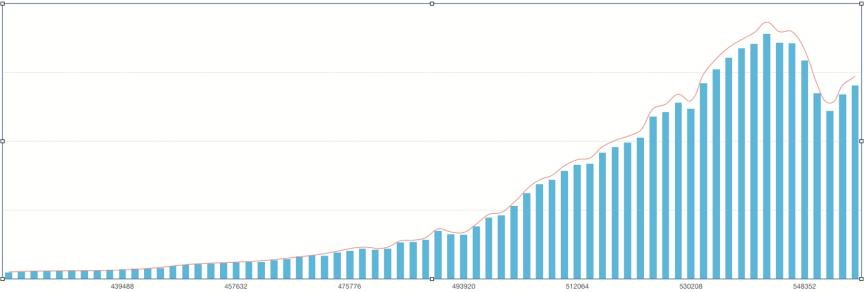
\includegraphics[width=10cm]{imagens/grafico3-capitulo-05.jpg}
  \caption{Hash Rate em relação a dificuldade}
\end{figure}

Como há uma defasagem de 2016 blocos entre os ajustes de dificuldade, é possível que haja picos massivos de aumento ou diminuição na \textit{hash rate} para mais ou menos produção de Bitcoin durante o período e isso pode violar levemente o cronograma da emissão. Na verdade, estamos um pouco mais rápidos agora em comparação com a meta original de finalizar a emissão em 2140. Como adicionar \textit{hash rate} normalmente significa produzir uma grande quantidade de novo hardware, isso é relativamente incomum e não afeta muito as coisas, e esperamos que isso se mantenha assim no futuro.

%no meu livro tem o topico Hashrate and the dollar value of bitcoin 
%e o topico fees and the end of block rewards

Quase concluímos a invenção de todo o Bitcoin:

\begin{enumerate}
\item Substituiu um banco central por um livro razão distribuído;
\item Instituiu um sistema de loteria para selecionar quem escreve no livro-razão;
\item Os participantes da loteria são forçados a consumir energia para comprar bilhetes por hash e torna mais fácil para todos poderem verificar os bilhetes vencedores, verificando os números hash produzidos pelos jogadores;
\item Diz aos jogadores da loteria que se eles não jogarem de acordo com as regras, rejeitamos os blocos, incluindo as \textit{transações de criação de moedas}, chamadas de \textit{coinbase}, para que eles não fossem pagos quando ganhassem, criando assim um desincentivo econômico para trapacear e um incentivo econômico para jogarem de acordo com as regras;
\item Controlou o tempo e a seleção do \textit{Alvo} para a loteria, permitindo que todos calculassem por si mesmos qual o \textit{Alvo} deveria ser, baseado nas regras codificadas e no histórico dos últimos 2016 blocos;
\item Aplicou o cronograma de emissão usando ajustes de dificuldade que são alterados de acordo com o aumento ou diminuição da \textit{hash rate};
\item Usou o código-fonte aberto para garantir que todos pudessem verificar por si mesmos se estavam aplicando as mesmas regras em relação à validade da transação, recompensa do bloco e cálculo de dificuldade.
\end{enumerate}

%isso esse paragrafo nao tem na minha versao(tirando a primeira e segunda frase(no qual mudei de posição)
% Qualquer um pode participar. Qualquer um pode jogar na loteria e criar bitcoins para si mesmo. Qualquer pessoa pode usar. A produção honesta de blocos é validada por toda a rede e recompensada com uma transação de \textit{coinbase} que paga ao minerador, ou punida por falta de recompensa e o minerador precisa consumir energia na mineração.
 
Não há mais entidade centralizada. Temos um sistema totalmente distribuído e descentralizado.
Quase temos a imagem completa do funcionamento da rede. Resta apenas um problema. Quando alguém se junta à rede e pede cópias do livro-razão, eles podem obter diferentes históricos de nodes diferentes. Como podemos impor uma história única e linear e como podemos evitar que os mineradores reescrevam o passado?